\documentclass[12pt,letterpaper]{article}
\usepackage{natbib}

%Packages
\usepackage{pdflscape}
\usepackage{fixltx2e}
\usepackage{textcomp}
\usepackage{fullpage}
\usepackage{float}
\usepackage{latexsym}
\usepackage{url}
\usepackage{epsfig}
\usepackage{graphicx}
\usepackage{amssymb}
\usepackage{amsmath}
\usepackage{bm}
\usepackage{array}
\usepackage[version=3]{mhchem}
\usepackage{ifthen}
\usepackage{caption}
\usepackage{hyperref}
\usepackage{amsthm}
\usepackage{amstext}
\usepackage{enumerate}
\usepackage[osf]{mathpazo}
\usepackage{dcolumn}
\usepackage{lineno}
\usepackage{dcolumn}
\newcolumntype{d}[1]{D{.}{.}{#1}}

\pagenumbering{arabic}


%Pagination style and stuff
\linespread{2}
\raggedright
\setlength{\parindent}{0.5in}
\setcounter{secnumdepth}{0} 
\renewcommand{\section}[1]{%
\bigskip
\begin{center}
\begin{Large}
\normalfont\scshape #1
\medskip
\end{Large}
\end{center}}
\renewcommand{\subsection}[1]{%
\bigskip
\begin{center}
\begin{large}
\normalfont\itshape #1
\end{large}
\end{center}}
\renewcommand{\subsubsection}[1]{%
\vspace{2ex}
\noindent
\textit{#1.}---}
\renewcommand{\tableofcontents}{}
%\bibpunct{(}{)}{;}{a}{}{,}

%---------------------------------------------
%
%       START
%
%---------------------------------------------

\newcommand{\disp}{\texttt{dispRity} }

\begin{document}

%Running head
\begin{flushright}
Version dated: \today
\end{flushright}
\bigskip
\noindent RH: dispRity package.

\bigskip
\medskip
\begin{center}

\noindent{\Large \bf \disp: a modular \texttt{R} package for measuring disparity.} 
\bigskip

\noindent {\normalsize \sc Thomas Guillerme$^1$$^,$$^*$}\\
\noindent {\small \it 
$^1$Imperial College London, Silwood Park Campus, Department of Life Sciences, Buckhurst Road, Ascot SL5 7PY, United Kingdom.\\}
\end{center}
\medskip
\noindent{*\bf Corresponding author.} \textit{guillert@tcd.ie}\\  
\vspace{1in}

%Line numbering
\modulolinenumbers[1]
\linenumbers

%---------------------------------------------
%
%       ABSTRACT
%
%---------------------------------------------

\newpage
\begin{abstract}

\begin{enumerate}
    \item We present \disp, an \texttt{R} package in multidimensional spaces. 
    \item Disparity designates a suit of metrics to describe an ordinated matrix (also referred as morpho/eco/niche/etc.-space).
    \item The package is based on a highly modular architecture were metrics for measuring disparity and tests for testing evolutionary hypothesis are provided as standalone functions.
    \item This modular architecture allows great plasticity in using this package, namely by letting users define their own metric of disparity.
    \item The package also provides numerous tools for modifying, summarising and plotting \disp objects.
\end{enumerate}

\end{abstract}

\noindent (Keywords: disparity, ordination, multidimensionality, disparity through time, palaeobiology, ecology)\\

\vspace{1.5in}

\newpage 

%---------------------------------------------
%
%       INTRODUCTION
%
%---------------------------------------------

\section{Introduction}

% Multidimensionality is a major aspect of natural sciences were variables co-vary through time and space from the organism to the environmental level.

% In palaeobiology multidimensionality is a popular way to study morphological diversity and comes as a interesting alternative to unidimensional taxonomic diversity analysis \citep{Hopkins2017}.

% Although the concept of morphological disparity is well defined since more than two decades \citep[e.g.][]{gould1991disparity,Foote01071994,Foote29111996}, its specific definition varies widely among authors.
% In fact disparity Disparity is by nature multidimensional \citep{lloyd2016estimating} and thus there are many ways to measure it.





%TG: rewrite all that using bits and blobs from previous intro
% Biological data are complex; understanding the ecology and evolution of species often requires that we analyse multiple variables that covary with each other, and through space and time.
% Multivariate analyses aim to capture and incorporate this multidimensional complexity, while providing outputs that are interpretable without needing to visualise n-dimensions simultaneously.
% Key multidimensional features of species that have important roles in ecology and evolution include morphology, functional traits. etc. etc.
% Many of these can be represented as matrices, these can be used in our package.
% In the interests of clarity/brievety, we here focus on just one kind of data: morphological diversity.

% In evolutionary biology and palaeontology, morphological diversity is often referred to as disparity.
% DESCRIBE COOL USES OF DISPARITY ANALYSES. WHY IS DISPARITY AWESOME.
% Although disparity is commonly studied, its definition varies widely across authors due to the myriad ways it can be measured.
% LIST WAYS IT IS MEASURED.
% This is further complicated by confusion over whether diparity refers to the metric describing or summarising one or more aspects of this space, or to the multidimensional space which is a specific mathematical object.
% This multidimensional space can also be defined in multiple ways.
% LIST ways

% In theory, this multitude of ways to measure/define disparity is not an issue. [the problem is that people aren't clear about it]
% The ideal solution is to choose either the most appropriate method for your question or data, or to apply several definitions and compare across these.[check biogeoBEARS]
% Unfortuantely, in practice this is hampered by existing software implementations.
% Package maintainers/software developers choose their preferred definition of disparity and method for measuring it, and then enforce this on users by allowing zero flexibility.
% This can lead to a chain of inappropriate analyses led by everyone just using the package that exists and the method within it, and in the worst case, using the defaults of the package. Oh no!
% The dispRity package will solve this problem by providing a completely flexible framework for studing disparity.
% It implements all commonly used metrics and definitions of disparity, as well as providing a simple interface for users to implement their own disparity functions.
% The package is described here for use with morphological diversity data, but the functions are equally applicable to ecological contexts such as Diaz paper, Deirdre's paper etc.






Biological data are complex; understanding the ecology and evolution of species often requires that we analyse multiple variables that covary with each other, and through space and time.
One solution to this problem is to analyse data in a multivariate framework.
Multivariate analyses aim to capture and incorporate this multidimensional complexity, while providing outputs that are interpretable in a physical world of only three dimensions.
Classical multidimensional species features that have been analysed through multivariate data ranges from their morphology \citep{raup1966geometric}, to their functional traits \citep{diaz2016global}.
However, such analysis are not limited at the species level and can also be applied to ecosystems \citep{DonohueDim}.

Key multidimensional features of species that have important roles in ecology and evolution include morphology, functional traits. etc. etc.
Many of these can be represented as matrices, these can be used in our package.
In the interests of clarity/brievety, we here focus on just one kind of data: morphological diversity.


Furthermore, we will also make a clear distinction between the multidimensional space which is a specific mathematical object and the disparity, which is a metric describing or summarising one or more aspects of this space.


Both can be defined in various ways depending on the authors, for example, disparity is defined as the weighted mean pairwise dissimilarity in \cite{Close2015} or the ellipsoid volume in \cite{DonohueDim} and the multidimensional space is defined as the morphospace in \cite{raup1966geometric} and the morpho-functional space in \cite{diaz2016global}.




The multidimensional space can be defined in many ways and arise from many mathematical transformations of the data such as the pairwise distance matrix \citep{Close2015}, a principal coordinates analysis \citep[PCO;][]{Brusatte12092008}, a principal components analysis \citep[PCA;][]{zelditch2012geometric}, a multidimensional scaling \citep[MDS;][]{DonohueDim}, etc.
Similarly, disparity metrics \citep[or indices;][]{Hopkins2017} can defined in many ways \citep[e.g.][or combinations thereof]{Wills2001,Ciampaglio2001,foth2012different,DonohueDim,Hughes20082013,finlay2015morphological,Close2015,diaz2016global}.
Finally, difference between disparity metrics can also be measured in many ways: using NPMANOVA \citep[e.g.][]{Brusatte12092008}, multidimensional permutation test \citep[e.g.][]{diaz2016global} or even simple confidence interval overlap \citep[e.g.][]{halliday2016eutherian}.

This variety of definitions and analysis have been developed in an equal variety of softwares such as \texttt{GINGKO} in javascript \citep{bouxin2005ginkgo,de2007ginkgo} or \texttt{geomorph} \citep{adams2013geomorph,adams2017geometric}, \texttt{Claddis} \citep{Claddis}, or \texttt{vegan} \citep{oksanen2007vegan} in R \citep{R}.
This results in the need to learn different languages (or at least - when restricted to R - different packages with different standards) as well as making analysis sometimes idiosyncratic and often complex to repeat since they are based on a particular feature from a particular software.
For example, in the excellent and widely used \texttt{geomorph} package morphological disparity analysis can be ran using the \texttt{morphol.disparity} function.
Unfortunately, however, the multidimensional space can only be defined as the ordination of the procrustes transform of geometric morphometric landmarks, the disparity can only be defined as the Procrustes variance and the difference between groups can only be measured through permutation tests \citep{zelditch2012geometric,adams2013geomorph,adams2017geometric}.

This package, is the first, to our knowledge, to be entirely dedicate to multidimensional analysis.
It has a highly modular architecture and allow users to define their own multidimensional space, use their own definition of the disparity metric and measure the differences between metrics in their own terms.
Furthermore, both a specific design and set of functions (through the \disp object) allows to design analysis into easy and repeatable pipelines.

\section{Description}
All the following functionalities of the package described below are based on the \disp class object.
This object class allows to repeat and streamline disparity analysis by being past from one function to the other (see Example section).
Specificities of the \disp object can be found in @@@ as well as series of utilities functions allowing to modify such object (see @@@).

\begin{table}
    \begin{tabular}{ll}
        \hline
        Function & Description \\ 
        \hline
        \texttt{geomorph.ordination} & Imports data from the \texttt{geomorph} package. \\
        \texttt{Claddis.ordination} & Imports data from the \texttt{Claddis} package. \\
        \texttt{custom.subsamples} & Separates ordinated data in custom subsamples. \\
        \texttt{time.subsamples} & Separates ordinated data in time subsamples. \\
        \texttt{boot.matrix} & Bootstraps and rarefies ordinated data or a \disp object. \\
        \disp & Calculates disparity from an ordinated matrix or a \disp object. \\
        \texttt{summary.dispRity} & Summarises a \disp object. \\
        \texttt{plot.dispRity} & Plots a \disp object. \\
        \texttt{test.dispRity} & Applies statistical tests to a \disp object.\\
        \texttt{dispRity.per.group} & Pipelined disparity per groups analysis. \\
        \texttt{dispRity.through.time} & Pipelined disparity through time analysis. \\
        \hline
    \end{tabular}
    \caption{Main functions in the \disp package.}
\end{table}


\subsection{Measuring disparity}
As hinted in the package name, the main functionality of this package is to measure disparity in a multidimensional space.
Again, within this package, disparity is defined as a description or a summary of one or more aspects of the multidimensional space.

The \disp function allows to measure disparity from any matrix (of class \texttt{matrix} or \texttt{data.frame}) where the columns correspond to the different dimensions of the multidimensional space (e.g. the ordination axis or any variable composing the space) and the rows correspond to the elements present in the multidimensional space (e.g. species, individuals, study sites, etc...).

Disparity can then be defined by the user as any function or combination of functions that can either transform the matrix into:
\begin{itemize}
    \item Another matrix (a Dimensions-level 3 function)
    \item A vector (a Dimensions-level 2 function)
    \item A single value (a Dimensions-level 1 function)
\end{itemize}

\begin{figure}[!htbp]
\centering
   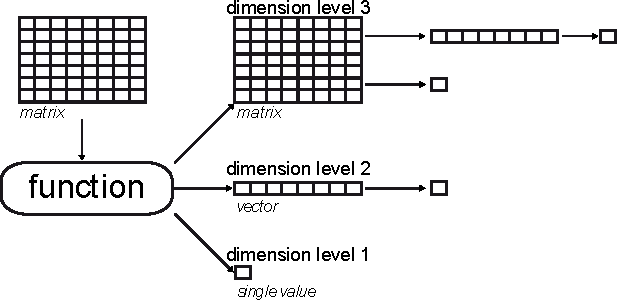
\includegraphics[width=1\textwidth]{../inst/gitbook/dispRity_fun.pdf} 
\caption{Illustration of the different metric dimensions levels in the \disp package}
\label{Fig:levels}
\end{figure}

The function(s) can then be passed to the \texttt{metric} argument to measure a specific aspect of the multidimensional space:
There is no limitation on the metric dimensions only that at least one dimensions level 2 or 1 are present in the definition (i.e. disparity can only be defined as distribution - a vector - or a single value).

Some metrics are implemented in the package

\begin{table}
\center
    \begin{tabular}{r|l|c|c|c}
        name & description & dimension level & definition & source \\
        \hline
        \texttt{ellipse.volume}$^1$ & The volume of the ellipsoid around the elements & 1 & $\frac{\pi^{k/2}}{\Gamma(\frac{k}{2}+1)}\displaystyle\prod_{i=1}^{k} (\lambda_{i}^{0.5})$ & \cite{DonohueDim}\\
        \texttt{convhull.surface} & The surface of the convex hull formed by the elements & 1 & NA & \texttt{geometry::convhulln} \\
        \texttt{convhull.volume} & The volume of the convex hull formed by the elements & 1 & NA & \texttt{geometry::convhulln} \\
        \texttt{hypervolume} & The volume of the multidimensional space space  & 1 & NA & \texttt{hypervolume::hypervolume} \\
        \texttt{diagonal} & The longest Eucliden distance between any pair of elements & 1 & $\sqrt{\sum_{i=1}^{k}|max(k_i) - min(k_i)|}$ & \texttt{dispRity::diagonal} \\
        \texttt{mode.val} & The modal value of a vector or a matrix & 1 & NA & \texttt{dispRity::mode.val}\\
        \texttt{ranges} & The absolute ranges of each dimension & 2 & $|max(k_i) - min(k_i)|$ & \texttt{dispRity::ranges} \\
        \texttt{variances} & The variance of each dimension & 2 & $\sigma^{2}{k_i}$ & \texttt{dispRity::variances} \\
        \texttt{centroids} & The distance between each element and a fixed point$^2$ of the space & 2 & $\sqrt{\sum_{i=1}^{n}{({k}_{n}-Centroid_{k})^2}}$ & \texttt{dispRity::centroids} \\
    \end{tabular}
    \caption{Where $k$ is the number of dimensions, $n$ the number of elements, $\lambda_i$ is the eigenvalue of each dimensions, $\sigma^{2}$ is their variance and $Centroid_{k}$ is their mean. $^1$ this function uses a fast estimation of the eigenvalue that only works in an ordinated space based on MDS or PCO/PCoA (\textit{not} PCA); $^2$ by default that point is the centroid of the elements.}
    \label{Tab:metrics}
\end{table}



\subsection{Splitting the multidimensional space into subsets}
A common analysis using multidimensional space consists into subdividing it into smaller samples, typically to compare to each other.
For example, one can be interested in looking how a specific sub-samples of the space compares in disparity from another (e.g. difference among groups) or, how different sub-samples change sequentially (e.g. through time).
In essence, the original multidimensional space (the input matrix) corresponds to overall space.
For example, if the multidimensional space is a morphospace, it corresponds to all the possible morphologies observed in the matrix.
Conversely, sub-samples of this space correspond to parts of the space with pooled characteristics.
For example, still in a morphospace with time sub-samples, each sub-samples correspond to all the observed morphologies during some time period.

These divisions can readily be created in the package using the \texttt{custom.subsamples} or \texttt{time.subsamples} functions.
The first takes as argument the matrix defining the multidimensional space and then a list of elements to group into different sub-samples.
The second also takes a multidimensional space and an additional argument on the age of the elements and then sorts them per time categories based on the following methods:

\begin{itemize}
    \item Discrete time subsamples: where the elements are grouped by age in time bins with corresponding ages.
    \item Continuous time subsamples: where the elements are defined as being the elements present at specific points in time (see @@@).
\end{itemize}

When using the \texttt{time.subsamples} function, it is also possible to provide a list of first and last occurence data for taxa spanning across specific time periods.
This allows species with a longer timespan to be present in multiple time sub-samples.

The continuous time sub-samples method works by using a phylogeny and looking at which taxa are present at any specific point in time.
This method thus requires a dated phylogeny (chronogram) and which model to use when slicing through branches rather than tips and nodes.

The slicing works by selecting any tips (and nodes if \texttt{inc.nodes = TRUE}) at the specific time slice.
When a slice occurs not on a tip or a node, four methods are available to select either the descendent or the ancestor's node/tip as an element for this time slice.
The models are:
\begin{itemize}
    \item ``acctran'' (accelerated transformation) where the data chosen along the branch is always the one of the descendant
    \item ``deltran'' (delayed transformation) where the data chosen along the branch is always the one of the ancestor
    \item ``punctuated'' where the data chosen along the branch is randomly chosen between the descendant or the ancestor
    \item ``gradual'' where the data chosen along the branch is either the descendant or the ancestor depending on branch length
\end{itemize}

\subsection{Bootstrapping and rarefying}
When measuring disparity, it is important to take sampling into account: for example, observed disparity in the whole multidimensional space can simply due to factors like the specific selection of elements (both their number or the presence of outliers).
To take these sources of error into account, it is common practice to bootstrap the data (to minimise the effect of outliers) or/and to rarefy the data (to minimise the effect of different sample sizes in different sub-samples).

\subsubsection{Bootstraps}
In disparity analysis, if disparity is defined as a dimension-level 1 metric (i.e. a metric summarising the multidimensional space into a single value), it can be useful to bootstrap this value in order to have a distribution on which to perform statistical analysis.
This can be achieved by using the \texttt{boot.matrix} function pseudo-replicates the multidimensional space following these two algorithms:

\begin{itemize}
    \item ``full'' algorithm: where the bootstrapping is entirely stochastic ($n$ elements are replaced by any $m$ elements drawn from the data)
    \item ``single'' algorithm: where only one random element is replaced by one other random element for each pseudo-replicate
\end{itemize}

\noindent Note that the ``single'' algorithm is somewhat akin to jackknife re-sampling where one element is duplicated rather than removed.

In the case of disparity being a dimension-level 1 metric, it is important to note that the distribution resulting from a bootstrap will be a pseudo-replicated one and thus might not be suitable for some specific parametric statistical tests.
Conversely, it is possible to use a dimension-level 2 metric on a bootstrapped multidimensional space to avoid this problem: the disparity metric is then measured on a pseudo-replicated multidimensional space rather than the metric itself being pseudo-replicated.

\subsubsection{Rarefactions}
The same \texttt{boot.matrix} function also allows to rarefy the multidimensional space or its sub-samples.
Rarefaction can be useful if, for example, one is interested in looking at the effect of reducing the number of elements on the results of an analysis or for allowing the comparisons of sub-samples wit the same number of elements in each.
In practice, rarefaction allows users to set a limit to the number of elements to be drawn for each bootstrap replication: only $n-x$ elements are selected at each bootstrap replicate (where $x$ is the number of non-sampled elements).

Additionally, this argument, is set to \texttt{TRUE} also allows to fully rarefy the sub-samples (i.e. removing $x$ elements for the number of pseudo-replicates, where *x* varies from the maximum number of elements present in each subsample to a minimum of three elements).

\subsection{Interpreting results}
Once disparity has been calculated (without or without sub-sampling, bootstrapping and rarefaction), the resulted \disp object can be summarised or plotted using the \texttt{S3} method functions \texttt{summary.dispRity} and \texttt{plot.dispRity}.
Finally, the results can be analysed using the \texttt{test.dispRity} function.

\subsubsection{Summary and plot}
The summary and plot functions allow to summarise the contents of the \disp objects.
These functions take as common arguments which central tendency (e.g. if central tendency is the mean and disparity was calculated as the sum of the variances for each dimensions, the central disparity tendency would be the mean of the sum of the variances) and the quantiles to represent (in the same example, if the quantile chosen is the 50th, these functions will also display 50\% of the sum of variances around the mean).

Additionally, the \texttt{plot.dispRity} function allows to graphically represent the summarised results using different representations:

\begin{itemize}
    \item ``continuous'' for displaying continuous disparity curves (in the case of disparity through time analysis for example)
    \item ``box'', ``lines'', or ``polygons'' to display discrete disparity results in respectively a boxplot, confidence interval lines, and confidence interval polygons.
\end{itemize}

Additional arguments can also be used such as \texttt{observed} to display the observed disparity (i.e. non-bootstrapped), \texttt{add} to add the plot in the current quartz window, or \texttt{rarefaction} to only plot the disparity for a specific number of elements and of course, any other normal graphical options can also be passed to this function (\texttt{main}, \texttt{xlab}, \texttt{col}, etc...).
Note that if the disparity has been calculated on fully rarefied data (using \texttt{boot.matrix(data, rarefaction = TRUE)} prior to calculating disparity), the rarefaction curves for the whole multidimensional space (or its sub-samples) can be plotted using \texttt{rarefaction = ``plot''}.

\subsubsection{test}
The \texttt{test.dispRity} function allows to test hypothesis on the disparity data (e.g. by comparing the different sub-samples between each other).
Similarly to the \disp function described above, this one can take any test defined by the user.
The \texttt{comparison} arguments allows to indicate in which order (if any) should the tests be applied:

\begin{itemize}
    \item ``pairwise'' for applying pairwise comparisons of all the subsamples (default).
    \item ``referential'' for comparing the first subsample to all the others.
    \item ``sequential'' for comparing each subsample sequentially (e.g. first against second, second against third, etc.).
    \item ``all'' for comparing all the subsamples simultaneously to the data (i.e. \texttt{disparity $\mathtt{\sim}$ subsamples}). This argument can be used for \texttt{lm} or \texttt{glm} type tests.
    \item or any list of pairs (or more) of number of sub-samples to compare (for example, for comparing the first to the sixth subsample and the fifth to the second: \texttt{comparison = list(c(1, 6), c(5, 2))})
\end{itemize}

Some tests are implemented within the package such as the Bhattacharrya Coefficient \citep[\texttt{bhatt.coeff}][]{Bhattacharyya,GuillermeCooper} or a permutation test based on null hypothesised multidimensional space following \cite{diaz2016global} (\texttt{null.test}).

This function also allows additionally argument such as \texttt{rarefaction} (as described above) or \texttt{correction} to adjust eventual p-values when multiple parametric tests are ran.

\section{Examples}
Here I provide to classic example of disparity analysis using some of the functions described above.
The data to reproduce these examples is available within the package and thus don't need to be downloaded:

\subsubsection{\disp data}
The package contains a dataset that is a subset from \cite{beckancient2014} including:

\begin{itemize}
    \item \texttt{BeckLee\_mat50}: an ordinated matrix for 50 mammals based on the distance between discrete morphological characters.
    \item \texttt{BeckLee\_mat99}: an ordinated matrix for the same 50 mammals as in \texttt{BeckLee\_mat50} but also containing the reconstruction of their 49 ancestors.
    \item \texttt{BeckLee\_tree}: a chronogram with the 50 mammals species present in \texttt{BeckLee\_mat50} and \texttt{BeckLee\_mat99}.
    \item \texttt{BeckLee\_ages}: the first and last occurrence data for 14 of the mammals species present in \texttt{BeckLee\_mat50} and \texttt{BeckLee\_mat99}.
    \item \texttt{disparity}: a pre-made \disp object based on the data above.
\end{itemize}

\subsubsection{Typical disparity through type analysis}

As an example, one can define their multidimensional space as being the morphospace of an ordination of the distance between discrete morphological characters for 50 mammals species \citep[from][]{beckancient2014}.
Then, one can define disparity as the sum of the variances on each dimensions \citep{Wills1994} that will represent an aspect of the the volume of the morphospace (i.e. a large sum of variances approximates a large morphospace).
One can then be interested in how this approximation of the volume of the morphospace changes throughout different time periods (say from the end of the Cretaceous to the end of the Palaeogene).

\texttt{disparity <- dispRity.through.time(data = BeckLee\_mat50, time = c(90, 70, 50, 30), metric = c(sum, variances))}
+ method = discrete
+ tree = tree

\noindent Note that this function is a wrapping function that is the equivalent to:

\texttt{disparity <- dispRity(boot.matrix(time.subsamples(data = BeckLee\_mat50, time = c(90, 70, 50, 30))), metric = c(sum, variances))}

\noindent Which allows a finer tuning of each optional argument in each of the three functions \texttt{time.subsamples}, \texttt{boot.matrix} and \disp.
The three arguments here are pretty self explanatory: \texttt{data = BeckLee\_mat50} is our definition of the multidimensional space, \texttt{time = c(90, 70, 50, 30)} indicates the boundaries of the different time bins and \texttt{metric = c(sum, variances)} is our definition of disparity.

This function returns a \disp object that does not directly gives us the results (the disparity in each time bin) but rather summarises the content of the \disp object.
To visualise the disparity values, one can use the \texttt{summary} or/and \texttt{plot} options:

\texttt{summary(disparity)}

\texttt{plot(disparity)}

% The `dispRity.through.time` function calculates disparity through time, a common analysis in palaeontology.
% This function (and the following one) uses an analysis pipeline with a lot of default parameters to make the analysis as simple as possible. 
% Of course all the defaults can be changed if required, more on this later.

% For a disparity through time analysis, you will need:
  
%   * An ordinated matrix (we covered that above)
%   * A phylogenetic tree: this must be a `phylo` object (from the `ape` package) and needs a `root.time` element. To give your tree a root time (i.e. an age for the root), you can simply do `my_tree\$root.time <- my\_age`.
%   * The required number of time subsamples (here `time = 3`)
%   * Your favourite disparity metric (here the sum of variances)

% Using the @beckancient2014 data described [above](#example-data):

% ## Measuring disparity through time
% disparity_data <- dispRity.through.time(BeckLee_mat50, BeckLee_tree,
%                                         time = 3, metric = c(sum, variances))
% ```

% This generates a `dispRity` object (see [here](#manipulating-dispRity-objects) for technical details).
% When displayed, these `dispRity` objects provide us with information on the operations done to the matrix:

% ```{r}
% ## Print the disparity_data object
% disparity_data
% ```

% We asked for three subsamples (evenly spread across the age of the tree), the data was bootstrapped 100 times (default) and the metric used was the sum of variances.

% We can now summarise or plot the `disparity_data` object, or perform statistical tests on it (e.g. a simple `lm`): 


% ```{r, fig.width=7, fig.height=7}
% ## Summarising disparity through time
% summary(disparity_data)

% ## Plotting the results
% plot(disparity_data, type = "continuous")

% ## Testing for an difference among the time bins
% disp_lm <- test.dispRity(disparity_data, test = lm, comparisons = "all")
% summary(disp_lm)

% ## Note that ANOVA assumptions were not checked here!
% ```

% Please refer to the [specific tutorials](#specific-tutorial) for (much!) more information on the nuts and bolts of the package.
% You can also directly explore the specific function help files within R and navigate to related functions.


\subsection{Typical disparity per groups analysis}

% The `dispRity.per.group` function is used if you are interested in looking at disparity among groups rather than through time.
% For example, you could ask if there is a difference in disparity between two groups?

% To perform such an analysis, you will need:
 
%  * An matrix with rows as elements and columns as dimensions (always!)
%  * A list of group members: this list should be a list of numeric vectors or names corresponding to the row names in the matrix. For example `list("a" = c(1,2), "b" = c(3,4))` will create a group _a_ containing elements 1 and 2 from the matrix and a group _b_ containing elements 3 and 4. Note that elements can be present in multiple groups at once.
%  * Your favourite disparity metric (here the sum of variances)

% Using the @beckancient2014 data described [above](#example-data):

% ```{r}
% ## Creating the two groups (crown versus stem) as a list
% mammal_groups <- list("crown" = c(16, 19:41, 45:50),
%                       "stem" = c(1:15, 17:18, 42:44))

% ## Measuring disparity for each group
% disparity_data <- dispRity.per.group(BeckLee_mat50, group = mammal_groups,
%                                      metric = c(sum, variances))
% ```

% We can display the disparity of both groups by simply looking at the output variable (`disparity_data`) and then summarising the `disparity_data` object and plotting it, and/or by performing a statistical test to compare disparity across the groups (here a Wilcoxon test).

% ```{r, fig.width=7, fig.height=7}
% ## Print the disparity_data object
% disparity_data

% ## Summarising disparity in the different groups
% summary(disparity_data)

% ## Plotting the results
% plot(disparity_data)

% ## Testing for a difference between the groups
% test.dispRity(disparity_data, test = wilcox.test, details = TRUE)
% ```




\section{Supplementary informations}
Supplementary information concerning each function's functionalities can be found in R in the individual function manuals as well as in the vignettes available online at @@@.


-Miscellaneous (maybe conclusion)
Simulations
Future directions




Conclusion


% \section{Data availability and reproducibility}
% Data are available on Dryad or Figshare.
% Code for reproducing the analyses is available on GitHub (\url{github.com/TGuillerme/SpatioTemporal_Disparity}).

\section{Acknowledgments}
Many thanks to Natalie Cooper for encouraging the development of this package and helping for the redaction of this paper and the package manuals.
Thanks to Dave Bapst, Martin Brazeau, Andrew Jackson, Graeme Lloyd and Emma Sherratt for specific implementation ideas.
I acknowledge support from European Research Council under the European Union's Seventh Framework Programme (FP/2007 – 2013)/ERC Grant Agreement number 311092 awarded to Martin D. Brazeau.

\section{Funding}
This work was funded by the European Research Council under the European Union's Seventh Framework Programme (FP/2007–2013)/ERC Grant Agreement number 311092.

\bibliographystyle{sysbio}
\bibliography{References}

\end{document}
